\chapter{Практическая часть}
\lstset{language=prolog}

В этом разделе будет описано задание данной работы и его решение.

\section{Условие}
Составить программу~--– базу знаний, с помощью которой можно определить, например, множество студентов, обучающихся в одном ВУЗе. Студент может одновременно обучаться в нескольких ВУЗах. Привести примеры возможных вариантов вопросов и варианты ответов (не менее 3-х). Описать порядок формирования вариантов ответа. При этом:
\begin{itemize}
    \item исходную базу знаний сформировать с помощью фактов;
    \item исходную базу знаний сформировать, используя правила;
    \item разработать свою базу знаний.
\end{itemize}

\section{База знаний}
В листинге~\ref{lst:knowledge} приведена база знаний, которая удовлетворяет условию задачи.
\begin{lstlisting}[caption={База знаний},label=lst:knowledge]
domains
  person, institution, country = symbol.
predicates
  university(institution, country).
  student(person, institution).

  studies_in(person, country).
  is_crossed(institution, institution).

clauses
  university(bmstu, russia).
  university(msu, russia).
  university(hse, russia).

  university(mit, usa).
  university(berkley, usa).
  university(harvard, usa).

  university(tum, germany).
  university(tub, germany).

  student(michael, hse).
  student(michael, tum).
  student(dmitry, bmstu).
  student(alexander, hse).
  student(artem, bmstu).
  student(artem, berkley).
  student(john, mit).
  student(nial, harvard).

  studies_in(Smb, Ctry) :-
    student(Smb, Usty),
    university(Usty, Ctry).

  is_crossed(Usty1, Usty2) :-
    student(Smb, Usty1),
    student(Smb, Usty2),
    not(Usty1 = Usty2).
\end{lstlisting}

Имеем домены:
\begin{itemize}
    \item person~--- человек;
    \item institution~--- учреждение;
    \item country~--- страна.
\end{itemize}

Имеем предикаты:
\begin{itemize}
    \item university(I: institution, C: country)~--- утвердение, что некоторое учреждение I, расположенное в некотором государстве C, является университетом;
    \item student(P: person, I: institution)~--- утверждение, что некоторое учреждение I является университетом, а некоторый человек P обучается в этом университете;
    \item studies\_in(P: person, C: country)~--- утверждение, что некоторый человек P обучается в университете, который расположен в некоторой стране C;
    \item is\_crossed(I1: institution, I2: institution)~--- утверждение, что два данных учреждения I1 и I2 являются университетами и в этих университетах есть хотя бы один общий студент.
\end{itemize}

\section{Цели}
Цель системы состоит в том, чтобы найти в базе знаний такое решение, исходя из которого на поставленный вопрос можно ответить <<да>>. Таких решений может быть несколько. В этом случае решение цели называют недетрминированным.

В листинге~\ref{lst:goal1} приведём текст цели, ищущей ответ на вопрос <<В каком университете учится dmitry?>>.
\begin{lstlisting}[caption={Цель \textnumero1},label=lst:goal1]
goal
  student(dmitry, Usty).
\end{lstlisting}
На рисунке~\ref{img:goal1} изображено решение этой цели. Оно не детерминировано.
\begin{figure}[H]
    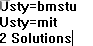
\includegraphics[scale=0.75]{imgs/goal1.png}
    \caption{Решение цели \textnumero1}\label{img:goal1}
\end{figure}

В листинге~\ref{lst:goal2} приведём текст цели, ищущей ответ на вопрос <<mit~--- университет?>>.
\begin{lstlisting}[caption={Цель \textnumero2},label=lst:goal2]
goal
  university(mit, _).
\end{lstlisting}
На рисунке~\ref{img:goal2} изображено решение этой цели.
\begin{figure}[H]
    
\includegraphics[scale=0.75]{imgs/goal2.png}
    \caption{Решение цели \textnumero2}\label{img:goal2}
\end{figure}

В листинге~\ref{lst:goal3} приведём текст цели, ищущей ответ на вопрос <<Кто учится в russia?>>.
\begin{lstlisting}[caption={Цель \textnumero3},label=lst:goal3]
goal
  studies_in(Smb, russia).
\end{lstlisting}
На рисунке~\ref{img:goal3} изображено решение этой цели. Оно не детерминировано.
\begin{figure}[H]
    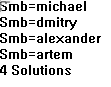
\includegraphics[scale=0.75]{imgs/goal3.png}
    \caption{Решение цели \textnumero3}\label{img:goal3}
\end{figure}

В листинге~\ref{lst:goal4} приведём текст цели, ищущей ответ на вопрос <<Какие университеты имеют общих студентов?>>.
\begin{lstlisting}[caption={Цель \textnumero4},label=lst:goal4]
goal
  is_crossed(Usty1, Usty2).
\end{lstlisting}
На рисунке~\ref{img:goal4} изображено решение этой цели. Оно не детерминировано.
\begin{figure}[H]
    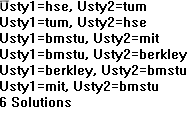
\includegraphics[scale=0.75]{imgs/goal4.png}
    \caption{Решение цели \textnumero4}\label{img:goal4}
\end{figure}

